\documentclass[conference]{IEEEtran}
\IEEEoverridecommandlockouts
\usepackage{cite}
\usepackage{amsmath,amssymb,amsfonts}
\usepackage{algorithmic}
\usepackage{graphicx}
\usepackage{textcomp}
\usepackage{xcolor}
\usepackage{booktabs}
\usepackage{array}
\usepackage{url}
\usepackage[hidelinks]{hyperref}
\def\BibTeX{{\rm B\kern-.05em{\sc i\kern-.025em b}\kern-.08em
    T\kern-.1667em\lower.7ex\hbox{E}\kern-.125emX}}

\begin{document}

\title{Levers and Indicators: A Guideline-Sourced Dependency Graph for Counterfactual Recourse in Diabetes Risk Prediction}

\author{\IEEEauthorblockN{Van Thieu and Phuc Do\textsuperscript{*}}
\IEEEauthorblockA{University of Information Technology, Ho Chi Minh City, Vietnam\\
Vietnam National University, Ho Chi Minh City, Vietnam\\
Email: vantv.20@grad.uit.edu.vn, \textsuperscript{*}phucdo@uit.edu.vn (corresponding author)}
}

\maketitle

\begin{abstract}
Counterfactual explanations are increasingly presented to clinicians as candidate intervention recommendations. A recommendation, unlike an explanation, must name something the patient can do. Knowledge-guided counterfactual methods enforce this partially, by declaring which features are immutable and in which direction each remaining feature may move. Direction, however, is not agency. A feature can be mutable, can move in the clinically desirable direction, and still not be an action: self-rated general health is not something a patient performs. We audit a peer-reviewed clinical counterfactual pipeline for diabetes risk and find that 11.0\% of its 1{,}000 counterfactuals recommend no action the patient can take, and that 22.3\% of all recommended feature changes target self-reported health-status indicators. Its own actionability metric scores every one of these at a violation rate of 0.000. The finding is stable across the five random seeds of that paper's own multi-seed protocol. The gaming-versus-improvement distinction that explains this behaviour is known, but existing treatments require a structural causal model, which health-survey instruments do not identify. We therefore recast the flat per-feature knowledge layer as a directed dependency graph in which direction is a node attribute and intervention route is an edge, with every edge sourced from a numbered recommendation of the ADA Standards of Care and carrying the evidence grade the ADA assigned to it. Removing indicators from the search space eliminates all unsupported recommendations at no cost to validity, which improves in five of five seeds.
\end{abstract}

\begin{IEEEkeywords}
counterfactual explanations, algorithmic recourse, clinical knowledge graph, actionability, diabetes risk prediction
\end{IEEEkeywords}

\section{Introduction}
Counterfactual explanations answer a question of the form: what would have had to be different for this prediction to change? In clinical decision support they are rarely consumed as explanations alone. They are surfaced to a clinician, and through the clinician to a patient, as \emph{candidate intervention recommendations}~\cite{thieu2026}. That reframing quietly imports an obligation the explanation literature does not owe: a recommendation must name an \textbf{action}.

Off-the-shelf counterfactual generators do not know what an action is. They perturb features until the prediction flips. Applied to observational health-survey data, where correlations arise as much from care-seeking behaviour as from physiology, this produces recommendations that are mathematically valid and clinically absurd. The best-known example, and the one that motivated the system we audit here, is a counterfactual that lowers predicted diabetes risk by advising the patient to skip their cholesterol check~\cite{thieu2026}.

Knowledge-guided counterfactual methods close part of this gap. They encode clinical domain knowledge as a constraint layer over the generator: a per-feature rule declaring which features are immutable and, for the rest, the direction in which a clinically appropriate intervention would move them. Physical activity may only increase; smoking may only decrease. The approach is a practical alternative to structural causal modelling when no structural causal model is identifiable, and it works: the system we audit raises its actionability score from 0.6655 to 0.9880 and drives wrong-direction violations to zero~\cite{thieu2026}.

\textbf{Direction, however, is not agency.} A feature may be mutable, may move in the direction the guidelines endorse, and still fail to be an action. Consider \texttt{GenHlth}, the BRFSS item that asks the respondent to rate their general health from excellent to poor. A counterfactual that advises \texttt{GenHlth: 5}$\rightarrow$\texttt{2} is telling the patient to feel considerably healthier. That is a description of a desired \emph{outcome}. It is not an \emph{intervention}. The distinction is orthogonal to mutability and orthogonal to direction, which is precisely why a direction-only rule table cannot see it.

This paper makes four claims. \textbf{First}, the failure mode is present, at scale, in a published and peer-reviewed clinical counterfactual pipeline, and its own actionability metric certifies it. Reproducing the released pipeline, we find that of 1{,}520 recommended feature changes across 200 high-risk patients, 350 (23.0\%) target self-reported health-status indicators, and 110 of 1{,}000 counterfactuals (11.0\%) recommend nothing the patient can act on at all. Every one is scored with a violation rate of 0.000. The audited system suppresses three features from its search space on the explicit grounds that they are \emph{healthcare-utilisation indicators and behavioural self-report features} whose association with diabetes is a selection effect rather than a causal pathway. Self-rated general health is also a self-reported health-status indicator. The system's own principle, applied consistently, excludes it. The system does not apply it.

\textbf{Second}, the conceptual distinction that explains this is not new, and we do not claim it. Miller et al.~\cite{miller2020} separate actions that change the prediction from actions that change the outcome; K\"onig et al.~\cite{konig2023} build Improvement-Focused Causal Recourse on that separation, with a motivating example structurally identical to ours: intervening on symptoms changes the diagnosis but not the infection. Their solution is correct and it requires a structural causal model, or at minimum a causal graph together with causal sufficiency, neither of which a health-survey instrument such as BRFSS provides~\cite{konig2023,thieu2026}. \textbf{The contribution here is to ask what can be done in that gap.}

\textbf{Third}, we recast the flat per-feature knowledge layer as a directed dependency graph. Direction remains a node attribute. A second node attribute records the feature's \textbf{role}: lever, treatable, indicator, or immutable. Edges assert that acting on one feature is a recognised route to changing another. The graph is deliberately weaker than a causal graph: it supports no do-calculus, estimates no interventional distribution, and assumes no causal sufficiency. It supports exactly one query, which is the only one the audit needs: \emph{is there a guideline-recognised route from any lever this counterfactual changes to the indicator it wants to move?} Every edge cites a numbered recommendation of the ADA Standards of Care and carries the evidence grade the ADA Professional Practice Committee assigned to it~\cite{ada2026s5,ada2026s8,ada2026s10,ada2026int}. No edge is inferred from BRFSS correlations, which would be circular: those correlations are what the generator is exploiting.

\textbf{Fourth}, enforcing the distinction is free. Excluding the three indicators from the generator's search space eliminates all unsupported recommendations and \textbf{improves} validity in five of five seeds (mean $+0.025$, paired $t=2.90$, $p=0.044$). The mechanism is visible in the data: counterfactuals that move an indicator without moving any lever have validity 0.614, against 0.861 for those that move a lever. The generator was using indicators as a cheap shortcut, and the shortcut was a poor one. Meanwhile the direction-only actionability score barely moves, from 0.980 to 0.975. It cannot distinguish a configuration that emits 110 meaningless recommendations from one that emits none. That is the argument for a different representation, and it is not an argument about performance.

\section{Background and Related Work}
\subsection{Counterfactual explanations as recourse}
Wachter et al.~\cite{wachter2017} introduced counterfactual explanations as the minimal perturbation that flips a prediction. DiCE~\cite{mothilal2020} generates diverse candidate counterfactuals for a single query. The reframing from explanation to \emph{recourse}, that is, from \emph{why} to \emph{what should I do}, is due to Ustun et al.~\cite{ustun2019} and Karimi et al.~\cite{karimi2021}, and it is the reframing that creates the problem this paper addresses: once a counterfactual is a recommendation, it acquires an obligation to be actionable.

\subsection{Constraining the action set}
The standard response is to restrict which features may vary and by how much. Ustun et al.~\cite{ustun2019} formalise this as an action set. FACE~\cite{poyiadzi2020} additionally requires that the counterfactual be reachable along the data manifold. FACEGroup~\cite{facegroup2025} builds a graph over instances, weighted by data density, to audit group fairness. Thieu~\cite{thieu2026} declares a per-feature intervention-direction taxonomy over BRFSS and translates it, per query, into the constraint interface of an off-the-shelf generator.

All of these share a shape: a rule attached to a feature, in isolation. The rule can say \emph{this feature may not move}, or \emph{this feature may only move upward}, or \emph{this feature may move within these bounds}. It cannot say \emph{this feature may only move as a consequence of moving that one}. That is a statement about a pair, and a flat table has no place to put it. FACEGroup's graph, in contrast, is over instances and is learned from data density; in our setting learning the graph from data would be circular, since the data correlations are precisely what the generator is exploiting.

\subsection{Gaming versus improvement, and why it needs a causal model}
Miller et al.~\cite{miller2020} observe that a predictive model creates an incentive structure, and separate two kinds of response to it: \textbf{gaming}, an action that changes the prediction without changing the underlying target, and \textbf{improvement}, an action that changes both. Shavit et al.~\cite{shavit2020} show that incentivising improvement, predictive accuracy, and recovering the true mechanism are in general in conflict.

K\"onig et al.~\cite{konig2023} carry this into recourse as Improvement-Focused Causal Recourse. Their motivating example is, structurally, ours: intervening on symptoms alters the diagnosis but not the infection, so a recourse method that optimises for acceptance may advise the patient to take cough drops. \textbf{We claim no novelty for this observation.} What we claim is that its remedy has been out of reach in our setting. ICR in its individualised form requires a fully specified structural causal model; in its subpopulation form it still requires the causal graph together with causal sufficiency, and the authors state plainly that SCMs and causal graphs are rarely readily available in practice~\cite{konig2023}. Their evaluation is conducted on synthetic and semi-synthetic structural causal models.

Health-survey instruments are exactly the case in which that requirement bites. BRFSS is a cross-sectional telephone survey; its variables are self-reported, temporally unordered, and confounded by care-seeking behaviour. The audited system adopted a flat rule table \textbf{because} no structural causal model was identifiable~\cite{thieu2026}. The question this paper asks is therefore not how to do causal recourse properly, which is settled, but \textbf{how little structure is enough to detect gaming when causal structure is unavailable.}

We also report an empirical contrast. K\"onig et al. find, on synthetic causal models, that improvement-focused actions cost more than gaming actions, because improvement requires more effort~\cite{konig2023}. In our clinical setting we find the opposite: suppressing the gaming shortcut costs nothing and improves validity in every seed we tested. The shortcut was not merely unactionable; it was also an inefficient way to flip the prediction.

\subsection{Knowledge graphs as evidence gates}
Knowledge graphs have been used both to reason over structured facts and to make clinical reasoning auditable. On the reasoning side, methods such as QUERY2TREE~\cite{query2tree2025} learn to answer logical queries over a knowledge graph by embedding its entities and relations. Our use is deliberately narrower and unlearned: CausalKG~\cite{causalkg2022} encodes interventional and counterfactual reasoning over a causal knowledge graph, while T2D-Bench~\cite{t2dbench2026} builds a multi-layer clinical-lifestyle knowledge graph, incorporating computable ADA Standards of Care rules, and uses it to \textbf{gate} the outputs of large language models against checkable evidence requirements. To our knowledge, no work applies this pattern to the output of a \textbf{counterfactual generator}. That is the narrow gap this paper occupies. We make no claim about the literature at large: graph-based counterfactual explanation is an established field with its own survey~\cite{pradoromero2024}. The claim is specific, and it is checkable: the recommendations a clinical counterfactual pipeline hands to a clinician have not been audited against a clinical knowledge graph.

\section{The Indicator-as-Lever Failure Mode}
\subsection{Levers and indicators}
We distinguish two roles a feature can play in a recourse recommendation. A \textbf{lever} is an upstream determinant the patient can act on directly. Body mass index, physical activity, smoking, fruit and vegetable intake are levers: there is something the patient does, and the feature moves as a result. An \textbf{indicator} is a downstream summary of health status. It reports rather than causes. In BRFSS, \texttt{GenHlth} asks the respondent to rate their general health on a five-point scale; \texttt{PhysHlth} and \texttt{MentHlth} ask how many of the past thirty days were physically or mentally unhealthy. A patient does not perform \texttt{GenHlth}. It is what happens to them.

The distinction is orthogonal to both axes a direction-only taxonomy encodes. An indicator is \textbf{mutable}: \texttt{GenHlth} can and does change. It has a \textbf{desirable direction}: lower is better. A rule table that records mutability and direction therefore admits it, and a violation metric defined over mutability and direction therefore certifies it. Nothing in that machinery has a place to record that the patient cannot pull the lever, because there is no lever. We call the resulting failure \textbf{indicator-as-lever recommendation}. Its conceptual root is the gaming/improvement distinction~\cite{miller2020,konig2023}; our contribution is to show that it survives, unnoticed and uncounted, inside a deployed clinical constraint layer.

\subsection{The audited system, and its own principle}
The system we audit~\cite{thieu2026} is a knowledge-guided counterfactual pipeline for BRFSS diabetes risk. Central to its contribution is the removal of three features from the search space entirely: \texttt{CholCheck}, \texttt{AnyHealthcare} and \texttt{HvyAlcoholConsump}. The stated rationale is that these behave as \emph{healthcare-utilisation indicators and behavioural self-report features}, whose correlation with diabetes reflects care-seeking patterns rather than a direct causal effect. The suppression accounts for 64\% of the paper's reported actionability gain. The principle is correct, and it is the paper's strongest idea. \textbf{The paper does not apply it consistently.} \texttt{GenHlth}, \texttt{PhysHlth} and \texttt{MentHlth} are also self-reported health-status indicators. They are retained, classified \texttt{monotonic\_down}, and left free for the generator to vary.

\subsection{The failure appears in the audited paper's own showcase}
The audited paper illustrates its contribution with a single high-risk patient. Table~\ref{tab:patient168} reproduces the comparison.

\begin{table}[t]
\caption{The audited system's own worked example (patient 168).}
\label{tab:patient168}
\centering
\footnotesize
\begin{tabular}{@{}p{1.4cm}p{3.1cm}p{2.6cm}@{}}
\toprule
\textbf{Mode} & \textbf{Recommendation} & \textbf{Verdict in \cite{thieu2026}} \\
\midrule
Unconstrained & Skip cholesterol check; lower income & Rejected as a search artefact \\
Direction-constrained & Lower cholesterol; \textbf{improve self-rated general health (\texttt{GenHlth} 5$\rightarrow$2)} & \textbf{Presented as the success case} \\
\bottomrule
\end{tabular}
\end{table}

The redirection is real, and the first recommendation is genuinely better than what it replaced. But the second component of the ``successful'' counterfactual instructs a patient to move their self-rated general health from \emph{poor} to \emph{very good}. That is the state the intervention is supposed to produce. It is not the intervention. The argument the paper uses to suppress \texttt{CholCheck} applies without modification to \texttt{GenHlth}.

\subsection{Why the metric cannot catch it}
The audited system scores each query with an actionability score, its Eq.~(1):
\begin{equation}
\mathrm{Act}(x_i) = 1 - \frac{V_{\mathrm{dir}}(x_i) + V_{\mathrm{imm}}(x_i)}{N_{\mathrm{changes}}(x_i)}
\end{equation}
where $V_{\mathrm{dir}}$ counts counterfactual changes that violate the taxonomy direction class of a feature, $V_{\mathrm{imm}}$ counts counterfactuals that alter any immutable feature, and $N_{\mathrm{changes}}$ is the total number of counterfactual feature changes for the query~\cite{thieu2026}. A recommendation to lower \texttt{GenHlth} from 5 to 2 violates neither term. It is not immutable, so it contributes nothing to $V_{\mathrm{imm}}$; its permitted direction is \texttt{monotonic\_down} and $5\rightarrow2$ moves downward, so it contributes nothing to $V_{\mathrm{dir}}$. It does, however, increment $N_{\mathrm{changes}}$. \textbf{An indicator-as-lever recommendation therefore does not merely escape the penalty. It inflates the denominator and thereby raises the score.} The metric is not miscalibrated, and the audited paper does not overstate it: it presents the score as a \emph{taxonomy-consistency proxy}, explicitly not a clinically validated actionability metric~\cite{thieu2026}. We take that disclaimer at face value and ask how wide the gap is in practice.

\section{$K_G$: A Guideline-Sourced Dependency Graph}
\subsection{From tuple to graph}
The knowledge layer of~\cite{thieu2026} is a set of per-feature tuples recording a direction class and a permitted range for each feature, independently of every other feature. A flat table has no slot in which to write \emph{this feature moves only as a consequence of moving that one}, because that is a statement about a pair. We define a directed graph $K_G = (V, E)$ with $V$ the twenty-one BRFSS features and $E$ a set of dependency edges. The direction class of~\cite{thieu2026} is retained verbatim as a node attribute, so that any difference in behaviour we report is attributable to what we add: a second node attribute, the feature's \textbf{role tier}, and the edge set.

\subsection{Role tiers}
Table~\ref{tab:tiers} gives the assignment. Four tiers answer one question: can the patient act on this, and how?

\begin{table}[t]
\caption{Role tiers over the twenty-one BRFSS features.}
\label{tab:tiers}
\centering
\footnotesize
\begin{tabular}{@{}p{1.5cm}p{4.2cm}p{1.3cm}@{}}
\toprule
\textbf{Tier} & \textbf{Features} & \textbf{Patient can act?} \\
\midrule
Lever & BMI, PhysActivity, Fruits, Veggies, Smoker, HvyAlcoholConsump, NoDocbcCost & Directly \\
Treatable & HighBP, HighChol & Via clinician \\
\textbf{Indicator} & \textbf{GenHlth, PhysHlth, MentHlth, DiffWalk} & \textbf{No} \\
Immutable / proxy & Age, Sex, Stroke, HeartDiseaseorAttack, Income, Education, AnyHealthcare, CholCheck & No \\
\bottomrule
\end{tabular}
\end{table}

\subsection{The decisive absence}
We searched sections 5, 8 and 10 of the ADA Standards of Care in Diabetes 2026~\cite{ada2026s5,ada2026s8,ada2026s10} for \textbf{any} numbered recommendation whose intervention target is self-rated general health, physically unhealthy days, or mentally unhealthy days. \textbf{There is none.} These constructs appear only as goals to be \emph{assessed}: Recommendation 5.3 directs the clinician to assess health status and well-being as key goals of self-management education~\cite{ada2026s5}. The section that would house such a recommendation is titled \emph{Facilitating Positive Health Behaviors and Well-being to Improve Health Outcomes}: behaviours are what one does, health outcomes are what improve as a result. The absence is the guideline-level justification for the indicator tier.

\subsection{Edges, and their evidence grades}
Every edge in $E$ asserts that acting on its source is a recognised route to changing its target, and cites a numbered ADA recommendation with the \textbf{evidence grade} the ADA Professional Practice Committee assigned to it~\cite{ada2026int}: A for adequately powered generalisable RCTs or meta-analyses; B for flawed trials or cohort and case-control studies; C for poorly controlled or observational studies; E for expert consensus. Grades are the committee's vote, not our judgment. The graph has 26 edges over 21 distinct source--target pairs: 12 at grade A, 3 at grade B, 3 at grade C, and 8 supported by section narrative rather than a numbered recommendation, which we mark separately as the weakest evidence. Table~\ref{tab:edges} gives the load-bearing edges.

\begin{table}[t]
\caption{Selected edges of $K_G$, with ADA evidence grades.}
\label{tab:edges}
\centering
\footnotesize
\begin{tabular}{@{}p{2.9cm}cp{2.4cm}@{}}
\toprule
\textbf{Edge} & \textbf{Grade} & \textbf{Source} \\
\midrule
PhysActivity $\rightarrow$ BMI & A & SoC'26 \S5, R5.12 \\
Fruits, Veggies $\rightarrow$ BMI & A & SoC'26 \S5, R5.12 \\
BMI $\rightarrow$ HighBP & A & SoC'26 \S8, R8.5 \\
BMI $\rightarrow$ HighChol & A & SoC'26 \S8, R8.5 \\
5 lifestyle levers $\rightarrow$ HighBP & A & SoC'26 \S10, R10.5 \\
PhysAct., Fruits, Veg. $\rightarrow$ HighChol & C & SoC'26 \S10, R10.15 \\
PhysActivity $\rightarrow$ GenHlth, PhysHlth, MentHlth & narr. & SoC'26 \S5 \\
BMI $\rightarrow$ GenHlth, PhysHlth & narr. & SoC'26 \S8 \\
\bottomrule
\end{tabular}
\end{table}

Recommendation 10.5, at grade A, is the single most load-bearing statement: one sentence names five lifestyle behaviours as routes to blood-pressure control, and yields five edges. Sections 8 and 10 carry external warrant: section 8 was approved by The Obesity Society, section 10 by the American College of Cardiology~\cite{ada2026int}. \textbf{No edge is inferred from BRFSS correlations}, which would be circular.

\subsection{What $K_G$ is not, and the audit rule}
$K_G$ is deliberately weaker than a causal graph. It licenses no do-calculus, estimates no interventional distribution, and assumes no causal sufficiency. It cannot say how much \texttt{GenHlth} will improve if BMI falls; it cannot even say that it will. It supports exactly one query, which is all the audit requires: given a counterfactual that changes a set of features $S$, and an indicator $v \in S$, does $S$ contain any lever $u$ with an edge $u \rightarrow v$ in $E$? This is a \textbf{necessary condition} for actionability, not a causal estimate. Formally, a change to $v$ is \textbf{unsupported} when
\begin{equation}
\mathrm{tier}(v){=}\mathrm{indicator} \;\wedge\; \{u : (u{\rightarrow}v){\in}E,\, \mathrm{tier}(u){=}\mathrm{lever},\, u{\in}S\} {=} \emptyset .
\end{equation}
This is the audit rule. It fits on one line, requires the edge set, and a flat table cannot express it.

\subsection{The graph structure}
Fig.~\ref{fig:kg} shows $K_G$. Reading the in-neighbourhoods of the indicator tier: \texttt{GenHlth}$\leftarrow\{$BMI, PhysActivity$\}$; \texttt{PhysHlth}$\leftarrow\{$BMI, PhysActivity, Smoker$\}$; \texttt{MentHlth}$\leftarrow\{$PhysActivity$\}$; \texttt{DiffWalk}$\leftarrow\emptyset$. There are exactly two guideline-recognised routes to improving self-rated general health, and they are the two most familiar levers in diabetes prevention. A counterfactual that asks a patient to improve \texttt{GenHlth} while touching neither is not merely optimistic; it has no path.

\begin{figure}[t]
\centering
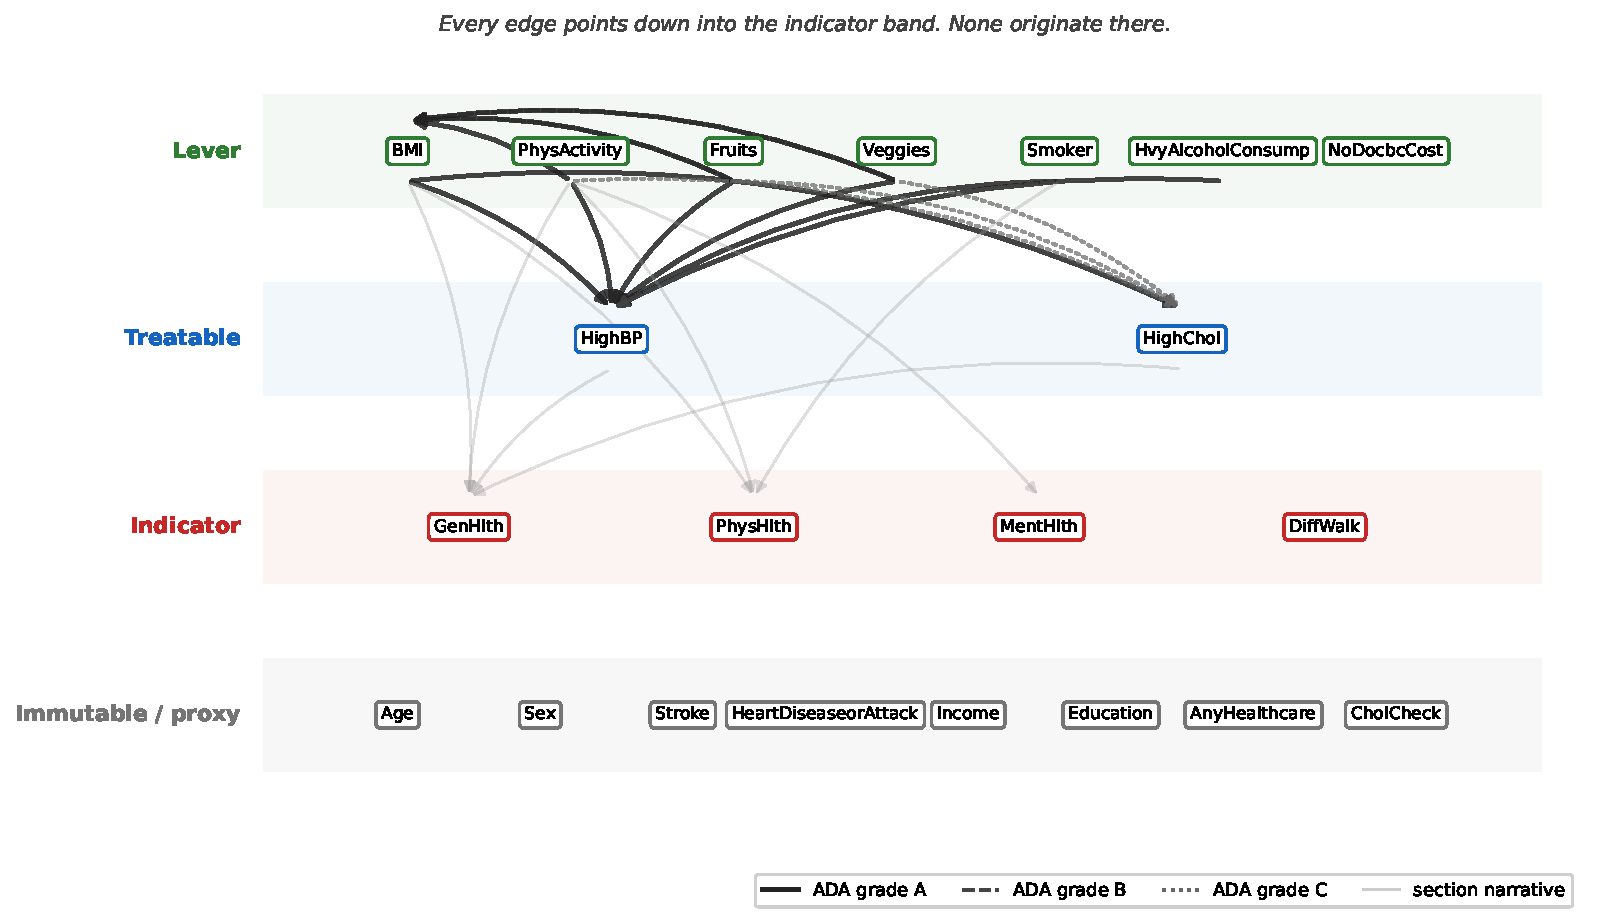
\includegraphics[width=\columnwidth]{fig1.pdf}
\caption{The knowledge graph $K_G$. Nodes are the 21 BRFSS features in four role bands; edges assert guideline-recognised intervention routes, with line style encoding the ADA evidence grade. Every edge points downward into the indicator band and none originates there: indicators are sinks. The immutable band is disconnected, lying on no intervention route.}
\label{fig:kg}
\end{figure}

\section{Audit: Applying $K_G$ to Published Counterfactuals}
\subsection{Setup and reproduction}
We reproduce the released pipeline of~\cite{thieu2026} without modification: the classifier, split, seed, cohort rule and DiCE backend are those of the published configuration, and the taxonomy source file is not touched. The only addition is that we record every counterfactual's feature-level changes, which the published pipeline aggregates away. Reproduction is faithful: test AUC 0.8234 against the published 0.8233, cohort mean risk 0.7495 against 0.7475, and 1{,}523 total counterfactual changes against 1{,}520. The residual 0.2\% arises from the stochastic \texttt{random} backend of DiCE across hardware and affects no conclusion. \textbf{No model is retrained and no counterfactual is regenerated for the audit.}

\subsection{Where the recommendations go}
Table~\ref{tab:audit} assigns each of the 1{,}523 recommended changes to a role tier.

\begin{table}[t]
\caption{Where the 1{,}523 recommended changes land (seed 42).}
\label{tab:audit}
\centering
\footnotesize
\begin{tabular}{@{}lrr@{}}
\toprule
\textbf{Tier} & \textbf{Changes} & \textbf{Share} \\
\midrule
Lever & 757 & 49.7\% \\
Treatable & 242 & 15.9\% \\
\textbf{Indicator} & \textbf{350} & \textbf{23.0\%} \\
Immutable / SES proxy & 174 & 11.4\% \\
\bottomrule
\end{tabular}
\end{table}

Slightly under half of what the system recommends is something the patient can do directly. \texttt{GenHlth} is the second most frequently recommended change in the entire system, behind only BMI: 128 of 200 patients (64\%) are told to raise their self-rated health by a mean of 2.32 categories on a 1--5 scale; \texttt{PhysHlth} 59/200 by a mean 15.73 of 30 days; \texttt{MentHlth} 34/200 by 12.19 days. Every one of these 350 changes is scored with a violation rate of 0.000.

\subsection{Applying the audit rule}
Applying the rule of Section IV-E to the 1{,}000 counterfactuals: 332 (33.2\%) change at least one indicator; of those, 171 (51.5\%) change no lever at all; \textbf{110 counterfactuals (11.0\%) recommend nothing the patient can act on whatsoever}, their changes falling exclusively on indicators and socioeconomic proxies; and 108 of 200 patients (54\%) receive at least one such counterfactual. Those 110 tell a patient, in effect, to be healthier and richer.

\subsection{What tempers this, and must be said}
\textbf{No patient receives five unactionable counterfactuals.} For every one of the 200 patients, at least one of the five is supported by a lever; a clinician reviewing the full set would find something usable for everyone. The failure is at the level of the individual counterfactual, not the patient. It matters nonetheless: a clinician is handed five candidate recommendations, presented as equivalently actionable by a metric reporting 0.988, and roughly one in nine cannot be carried out, with nothing marking which.

\subsection{Both readings, and robustness}
Placing \texttt{HighBP} and \texttt{HighChol} in the treatable tier is a judgment; a reviewer may hold they are downstream of BMI and belong with the indicators. Under the narrow reading (indicators only) non-lever recommendations are 350/1{,}523 (23.0\%); under the broad reading (indicators and treatables) 592/1{,}523 (38.9\%). The conclusion does not turn on the choice. The audit is also stable across the five seeds of the audited paper's own protocol $\{42, 123, 2024, 7, 31337\}$: indicator changes range 291--350, no-lever counterfactuals 160--178, and fully-unactionable counterfactuals 96--111. The 174 changes on \texttt{Income} and \texttt{Education} are not our finding: the audited paper already reports a conservative ablation making those immutable~\cite{thieu2026}. The novel axis is the indicator tier.

\section{Enforcement: What Does It Cost to Stop?}
\subsection{Configuration and result}
The graph predicts that removing \texttt{GenHlth}, \texttt{PhysHlth} and \texttt{MentHlth} from the generator's search space should cost nothing a patient could have used. We test this directly: the three indicators are excluded from \texttt{features\_to\_vary}, everything else identical. Table~\ref{tab:enforce} reports the mean over five seeds.

\begin{table}[t]
\caption{Published taxonomy versus $K_G$ constraint, mean of five seeds.}
\label{tab:enforce}
\centering
\footnotesize
\begin{tabular}{@{}lrr@{}}
\toprule
 & \textbf{Published} & \textbf{With $K_G$} \\
\midrule
Validity & 0.8012 & \textbf{0.8266} \\
Indicator changes & 291--350 & \textbf{0} \\
Unsupported counterfactuals & 160--178 & \textbf{0} \\
Patients left with no CF & 0/200 & 0/200 \\
Mean changes per CF & 1.52 & 1.48 \\
\textbf{Direction-only actionability} & \textbf{0.9804} & \textbf{0.9742} \\
\bottomrule
\end{tabular}
\end{table}

Validity improves in \textbf{five seeds out of five} (mean $+0.0254$, sd $0.0196$, paired $t=2.90$, $p=0.044$). The per-seed gain ranges from $+0.005$ to $+0.050$, so \textbf{we make no claim about the size of the improvement}; the defensible claim is that enforcing the lever/indicator distinction carries \textbf{no measurable validity cost}. No patient loses their counterfactual set.

\subsection{Why it is free, and the blind metric}
The mechanism is visible in the audit data. Counterfactuals that move an indicator without moving any lever have validity 0.614; those that move a lever have 0.861. The generator used indicators as a cheap perturbation that flipped the prediction poorly. Removing it forces the search onto levers, which work better. This runs against the closest prior result: K\"onig et al. report, on synthetic causal models, that improvement costs \emph{more} than gaming~\cite{konig2023}; on real survey data we find the opposite. We do not claim this generalises. The last row of Table~\ref{tab:enforce} is the reason this paper argues for a representation and not a hyperparameter: the direction-only actionability score is 0.9804 with 110 unactionable counterfactuals and 0.9742 with none. It moves by six thousandths, in the wrong direction. No tuning fixes this; the knowledge layer needs another axis, and the axis needs an edge.

\section{Limitations}
The lever/indicator boundary is a judgment, not a measurement; \texttt{HighBP} and \texttt{HighChol} are the contested cases and we report both readings. Edges are asserted from guideline recommendations and carry the ADA's grade, but no effect size is estimated and no edge is validated on data; learning them from BRFSS would be circular. Eight of the 26 edges rest on section narrative rather than a numbered recommendation, are marked as such, and all point into the indicator tier where the audit rule bites; the honest reason is that the ADA does not issue graded recommendations about self-rated health, because self-rated health is not a target of care, which is the point Section IV-C makes. No clinical panel reviewed our tiers; the audited paper concedes the same about its own class assignments, and ours inherit it. Results are for one cohort, one generator, one classifier (BRFSS 2021, DiCE, XGBoost). $K_G$ is not a causal model and makes no interventional claims; where a structural causal model is available, ICR~\cite{konig2023} is the stronger tool.

\section{Conclusion}
Direction was the right first axis for a clinical knowledge layer, and encoding it works: it removes the recommendation to skip a cholesterol check. It is not the last axis. A recommendation must not only point the right way; it must name something the patient can do. We showed that a peer-reviewed clinical counterfactual pipeline recommends, in 11\% of its counterfactuals, nothing the patient can act on, and that its own actionability metric certifies every one. The failure is invisible to a direction-only rule table because it is not about direction but about whether a route exists from an action to the thing being changed, and a route is an edge. Recasting the flat layer as a dependency graph, with every edge traceable to a graded clinical recommendation, makes the failure detectable in one query and eliminates it at no cost to validity. Where the causal model exists, use it. Where it does not, an edge is still better than a row.

\section*{Acknowledgment}
The reproduction package and the knowledge-graph module are available at the repository accompanying this paper.

\begin{thebibliography}{00}
\bibitem{thieu2026} V. Thieu, ``Knowledge-guided counterfactual explanations for diabetes risk decision support: a directional intervention taxonomy,'' \emph{Int. J. Med. Inform.}, vol. 219, art. 106555, 2026. \url{https://doi.org/10.1016/j.ijmedinf.2026.106555}
\bibitem{wachter2017} S. Wachter, B. Mittelstadt, and C. Russell, ``Counterfactual explanations without opening the black box: automated decisions and the GDPR,'' \emph{Harv. J. Law Technol.}, vol. 31, no. 2, pp. 841--887, 2017. \url{https://doi.org/10.2139/ssrn.3063289}
\bibitem{mothilal2020} R. K. Mothilal, A. Sharma, and C. Tan, ``Explaining machine learning classifiers through diverse counterfactual explanations,'' in \emph{Proc. ACM FAT* '20}, 2020, pp. 607--617. \url{https://doi.org/10.1145/3351095.3372850}
\bibitem{ustun2019} B. Ustun, A. Spangher, and Y. Liu, ``Actionable recourse in linear classification,'' in \emph{Proc. ACM FAT* '19}, 2019, pp. 10--19. \url{https://doi.org/10.1145/3287560.3287566}
\bibitem{karimi2021} A.-H. Karimi, B. Sch\"olkopf, and I. Valera, ``Algorithmic recourse: from counterfactual explanations to interventions,'' in \emph{Proc. ACM FAccT '21}, 2021, pp. 353--362. \url{https://doi.org/10.1145/3442188.3445899}
\bibitem{poyiadzi2020} R. Poyiadzi, K. Sokol, R. Santos-Rodriguez, T. De Bie, and P. Flach, ``FACE: feasible and actionable counterfactual explanations,'' in \emph{Proc. AAAI/ACM AIES '20}, 2020, pp. 344--350. \url{https://doi.org/10.1145/3375627.3375850}
\bibitem{facegroup2025} C. Fragkathoulas, V. Papanikou, E. Pitoura, and E. Terzi, ``FACEGroup: feasible and actionable counterfactual explanations for group fairness,'' in \emph{Proc. ECML PKDD}, 2025. \url{https://arxiv.org/abs/2410.22591}
\bibitem{miller2020} J. Miller, S. Milli, and M. Hardt, ``Strategic classification is causal modeling in disguise,'' in \emph{Proc. ICML}, 2020, pp. 6917--6926. \url{https://arxiv.org/abs/1910.10362}
\bibitem{shavit2020} Y. Shavit, B. Edelman, and B. Axelrod, ``Causal strategic linear regression,'' in \emph{Proc. ICML}, 2020, pp. 8676--8686. \url{https://arxiv.org/abs/2002.10066}
\bibitem{konig2023} G. K\"onig, T. Freiesleben, and M. Grosse-Wentrup, ``Improvement-focused causal recourse (ICR),'' in \emph{Proc. AAAI Conf. Artif. Intell.}, vol. 37, no. 10, 2023, pp. 11847--11855. \url{https://doi.org/10.1609/aaai.v37i10.26398}
\bibitem{query2tree2025} T. H. V. Phan and P. Do, ``QUERY2TREE: a reasoning model for answering logical queries based on knowledge graph embedding and large language model,'' \emph{Knowl. Inf. Syst.}, vol. 67, pp. 5271--5300, 2025. \url{https://doi.org/10.1007/s10115-025-02347-z}
\bibitem{causalkg2022} U. Jaimini and A. Sheth, ``CausalKG: causal knowledge graph explainability using interventional and counterfactual reasoning,'' \emph{IEEE Internet Comput.}, vol. 26, no. 1, pp. 43--50, 2022. \url{https://doi.org/10.1109/MIC.2021.3130675}
\bibitem{t2dbench2026} S. A. Farahani, H. Cao, R. Jain, and A. M. Rahmani, ``T2D-Bench: evidence-gated evaluation of LLM outputs for type 2 diabetes using a multi-layer clinical-lifestyle knowledge graph,'' arXiv preprint, 2026. \url{https://arxiv.org/abs/2606.24145}
\bibitem{pradoromero2024} M. A. Prado-Romero, B. Prenkaj, G. Stilo, and F. Giannotti, ``A survey on graph counterfactual explanations: definitions, methods, evaluation, and research challenges,'' \emph{ACM Comput. Surv.}, vol. 56, no. 7, pp. 1--37, 2024. \url{https://doi.org/10.1145/3618105}
\bibitem{ada2026s5} American Diabetes Association Professional Practice Committee, ``5. Facilitating positive health behaviors and well-being to improve health outcomes: Standards of Care in Diabetes 2026,'' \emph{Diabetes Care}, vol. 49, suppl. 1, pp. S89--S131, 2026. \url{https://doi.org/10.2337/dc26-S005}
\bibitem{ada2026s8} American Diabetes Association Professional Practice Committee, ``8. Obesity and weight management for the prevention and treatment of diabetes: Standards of Care in Diabetes 2026,'' \emph{Diabetes Care}, vol. 49, suppl. 1, 2026. \url{https://doi.org/10.2337/dc26-S008}
\bibitem{ada2026s10} American Diabetes Association Professional Practice Committee, ``10. Cardiovascular disease and risk management: Standards of Care in Diabetes 2026,'' \emph{Diabetes Care}, vol. 49, suppl. 1, pp. S216--S245, 2026. \url{https://doi.org/10.2337/dc26-S010}
\bibitem{ada2026int} American Diabetes Association Professional Practice Committee, ``Introduction and methodology: Standards of Care in Diabetes 2026,'' \emph{Diabetes Care}, vol. 49, suppl. 1, pp. S1--S5, 2026. \url{https://doi.org/10.2337/dc26-SINT}
\end{thebibliography}

\end{document}
